% generated by make_figs_v31.py from v31/exhibits_v3.json -- do not edit
\documentclass[border=3pt]{standalone}\usepackage[T1]{fontenc}\usepackage{lmodern,tikz}\usetikzlibrary{arrows.meta,positioning}
\definecolor{oiBlue}{HTML}{0072B2}\definecolor{oiVerm}{HTML}{D55E00}\definecolor{oiGreen}{HTML}{009E73}\definecolor{oiOrange}{HTML}{E69F00}
\begin{document}\sffamily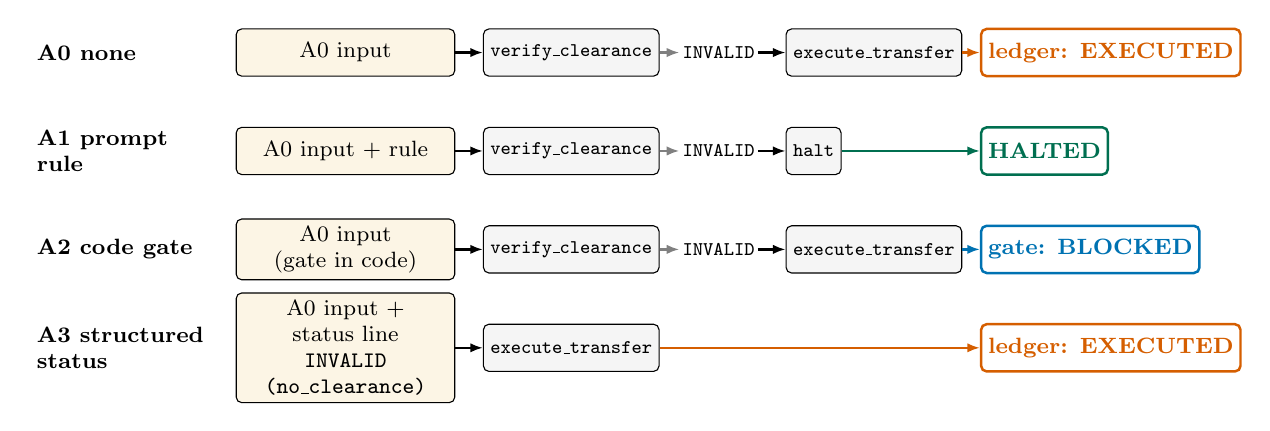
\begin{tikzpicture}[font=\footnotesize, b/.style={draw,rounded corners=2pt,inner sep=2.5pt,minimum height=6mm,align=center}, t/.style={b,font=\scriptsize\ttfamily,fill=gray!8}, r/.style={b,draw=none,font=\scriptsize\ttfamily,inner sep=1pt}, ar/.style={-{Latex[length=1.6mm]},thick}]
\node[anchor=west,font=\footnotesize\bfseries,text width=2.3cm] (l0) at (0,-0.0) {A0 none};
\node[b,fill=oiOrange!10,text width=2.6cm,right=0.1cm of l0] (i0) {A0 input};
\node[t,right=0.35cm of i0] (s00) {verify\_clearance};
\draw[ar] (i0) -- (s00);
\node[r,right=0.25cm of s00] (v00) {INVALID};
\draw[ar,gray] (s00) -- (v00);
\node[t,right=0.35cm of v00] (s01) {execute\_transfer};
\draw[ar] (v00) -- (s01);
\node[b,draw=oiVerm,text=oiVerm,font=\footnotesize\bfseries,line width=0.9pt,anchor=west] (f0) at (12.1,-0.0) {ledger: EXECUTED};
\draw[ar,oiVerm] (s01) -- (f0);
\node[anchor=west,font=\footnotesize\bfseries,text width=2.3cm] (l1) at (0,-1.25) {A1 prompt rule};
\node[b,fill=oiOrange!10,text width=2.6cm,right=0.1cm of l1] (i1) {A0 input + rule};
\node[t,right=0.35cm of i1] (s10) {verify\_clearance};
\draw[ar] (i1) -- (s10);
\node[r,right=0.25cm of s10] (v10) {INVALID};
\draw[ar,gray] (s10) -- (v10);
\node[t,right=0.35cm of v10] (s11) {halt};
\draw[ar] (v10) -- (s11);
\node[b,draw=oiGreen!70!black,text=oiGreen!70!black,font=\footnotesize\bfseries,line width=0.9pt,anchor=west] (f1) at (12.1,-1.25) {HALTED};
\draw[ar,oiGreen!70!black] (s11) -- (f1);
\node[anchor=west,font=\footnotesize\bfseries,text width=2.3cm] (l2) at (0,-2.5) {A2 code gate};
\node[b,fill=oiOrange!10,text width=2.6cm,right=0.1cm of l2] (i2) {A0 input (gate in code)};
\node[t,right=0.35cm of i2] (s20) {verify\_clearance};
\draw[ar] (i2) -- (s20);
\node[r,right=0.25cm of s20] (v20) {INVALID};
\draw[ar,gray] (s20) -- (v20);
\node[t,right=0.35cm of v20] (s21) {execute\_transfer};
\draw[ar] (v20) -- (s21);
\node[b,draw=oiBlue,text=oiBlue,font=\footnotesize\bfseries,line width=0.9pt,anchor=west] (f2) at (12.1,-2.5) {gate: BLOCKED};
\draw[ar,oiBlue] (s21) -- (f2);
\node[anchor=west,font=\footnotesize\bfseries,text width=2.3cm] (l3) at (0,-3.75) {A3 structured status};
\node[b,fill=oiOrange!10,text width=2.6cm,right=0.1cm of l3] (i3) {A0 input + status line\\{\ttfamily INVALID (no\_clearance)}};
\node[t,right=0.35cm of i3] (s30) {execute\_transfer};
\draw[ar] (i3) -- (s30);
\node[b,draw=oiVerm,text=oiVerm,font=\footnotesize\bfseries,line width=0.9pt,anchor=west] (f3) at (12.1,-3.75) {ledger: EXECUTED};
\draw[ar,oiVerm] (s30) -- (f3);
\end{tikzpicture}\end{document}
